\section{Introduction}
\label{sec:intro}

Large language models have demonstrated remarkable capabilities across a wide range of tasks, such as deep research~\citep{shao2025dr, openai2025deep}, software engineering tasks~\citep{jimenez2023swe, liu2025migrationbench, merrill2026terminal}, search and retrieval~\citep{jin2025search}, and user interaction~\citep{yao2024tau, barres2025tau}. Recently, the agentic paradigm has further extended these capabilities by equipping LLMs with external tools for complex planning, multi-step problem solving, and real-world interactions~\citep{schick2023toolformer, qin2023toolllm, patil2024gorilla}. However, current tool-augmented agents tend to call tools indiscriminately, even when the model already possesses the ability to answer directly. A central design question in these systems is therefore: \emph{when should the model call a tool versus solve the task directly?} In many cases, tool calls are unnecessary: an agent does not need to launch a web search or RAG pipeline to answer ``what year did humans land on the Moon?. Each unnecessary call wastes API fees, costs that compound rapidly when an agent makes dozens of decisions per session at deployment scale.

Recent work has begun to address tool-call efficiency, but existing approaches either target a different problem or bypass the question of \emph{why} models overcall. \citet{wu2025joint} reduces redundant calls by jointly refining agent instructions and tool descriptions, but focus on improving calls that are already needed, not on deciding whether a call is necessary. \citet{xu2025alignment} study when to skip tools entirely, but evaluate with oracle tools that simply return the correct answer upon invocation, and rely on SFT to modify behavior without understanding why the model overcalls. This leaves a fundamental question unanswered: \textit{do models overcall because they lack the information to decide, or because they fail to act on information they already have}?

Motivated by these limitations, we propose \benchmark{} (Section~\ref{sec:benchmark}), a benchmark designed to study the tool-call decision in a setting that closely mirrors real-world agent deployments. \benchmark{} comprises 18 environments (15 single-hop and 3 multi-hop), each providing tools that the model must invoke with correctly formatted arguments and whose responses require parsing, matching the interaction pattern of real APIs. We identify three categories of situations where an agent must decide whether to use a tool, covering what we believe are the major real-world scenarios: (1)~\emph{``Can I compute this?''}: the model understands the operation, but the operands may exceed what it can compute reliably (e.g. $12+7$ is trivial; trillion-scale multiplication is not); (2)~\emph{``Do I know this?''}: the answer may or may not exist in the model's parameters (e.g. the capital of France is common knowledge; an obscure historical date may not be); and (3)~\emph{``Can I execute this reliably?''}: the model knows the rules, but mentally tracing many sequential steps is error-prone (e.g. predicting \texttt{print(2+3)} is easy; tracing deep recursion might not). Each environment has three difficulty levels: \emph{easy} (most models can reliably solve without tools), \emph{medium} (the decision boundary where models sometimes succeed and sometimes fail), and \emph{hard} (most models cannot succeed without tools). Using \benchmark{}, we systematically evaluate two training-free baselines: Prompt-only, which varies the system prompt to discourage unnecessary calls, and Reason-then-Act, which asks the model to explicitly reason about tool necessity before acting. We find that both provide limited control over tool-call decisions, with hard tasks paying a high accuracy cost for each saved call (Section~\ref{sec:behavioral}).

Given the limited ability of prompting and reasoning, we ask a deeper question: \textit{does the model internally encode information about whether a tool is needed?} To investigate, we probe the model's hidden representations (Section~\ref{sec:probing}). We extract the hidden state at the last input token and train a simple linear classifier to predict whether a tool call is necessary. Surprisingly, the probe achieves AUROC above 0.9 across models. This reveals that \textbf{the model already encodes a clean signal about tool necessity in its hidden state}, but the generation process fails to translate it into calibrated decisions. Notably, even for models that completely fail under Reason-then-Act, the probe still extracts a strong signal, demonstrating that representation-level knowledge exists independently of the model's ability to express it through text.

Building on this finding, we propose \textbf{\method{}} (Section~\ref{sec:method}). We train a lightweight linear probe on the hidden states with binary tool-necessity labels. At inference time, the probe reads the hidden state and prefills the model's response with a short steering sentence (e.g., ``I can solve this directly without using a tool'' or ``I need to use a tool for this question''). The model then continues generating from this prefill. By adjusting the probe's decision threshold, \method{} provides smooth, fine-grained control over the accuracy--efficiency tradeoff. Across all tested models, \method{} outperforms every Prompt-only and Reason-then-Act baseline, and transfers well between tasks. It reduces unnecessary tool calls while preserving accuracy on hard tasks, requiring only a simple linear prediction and no additional reasoning from the model.

Our contributions are three-fold, progressing systematically from benchmark design and failure analysis, to a proposed mitigation method:
\begin{itemize}[leftmargin=*]
    \item \textbf{Benchmark:} We design \textbf{\benchmark{}}, the first benchmark for studying tool-call decisions. It comprises 18 environments (15 single-hop, 3 multi-hop) across three categories of tool necessity with controlled difficulty levels, totaling 1{,}080 training and 2{,}700 test tasks.
    \item \textbf{Failure Analysis:} We evaluate Prompt-only and Reason-then-Act baselines, revealing that both provide limited and coarse control over tool-call decisions, with hard tasks paying a disproportionate accuracy cost for each saved call.
    \item \textbf{Discovery \& Mitigation:} We probe pre-generation hidden states and find that tool necessity is linearly decodable. We therefore exploit this signal and propose \textbf{\method{}}, a lightweight method ($<$1ms overhead) that prefills the model's response based on the probe prediction. \textbf{\method{}} reduces tool calls by 48\% with only 1.7\% accuracy loss, while the best baselines either reduce tool calls by only 6\% at comparable accuracy (i.e. 8$\times$ less efficient) or suffer 5$\times$ more accuracy loss for a similar reduction. Furthermore, our method generalizes to real-world agentic search, reducing API calls by 20--56\% on the Search-o1 agentic benchmark \citep{li2025search}.
\end{itemize}


\begin{figure*}[t!]
\centering
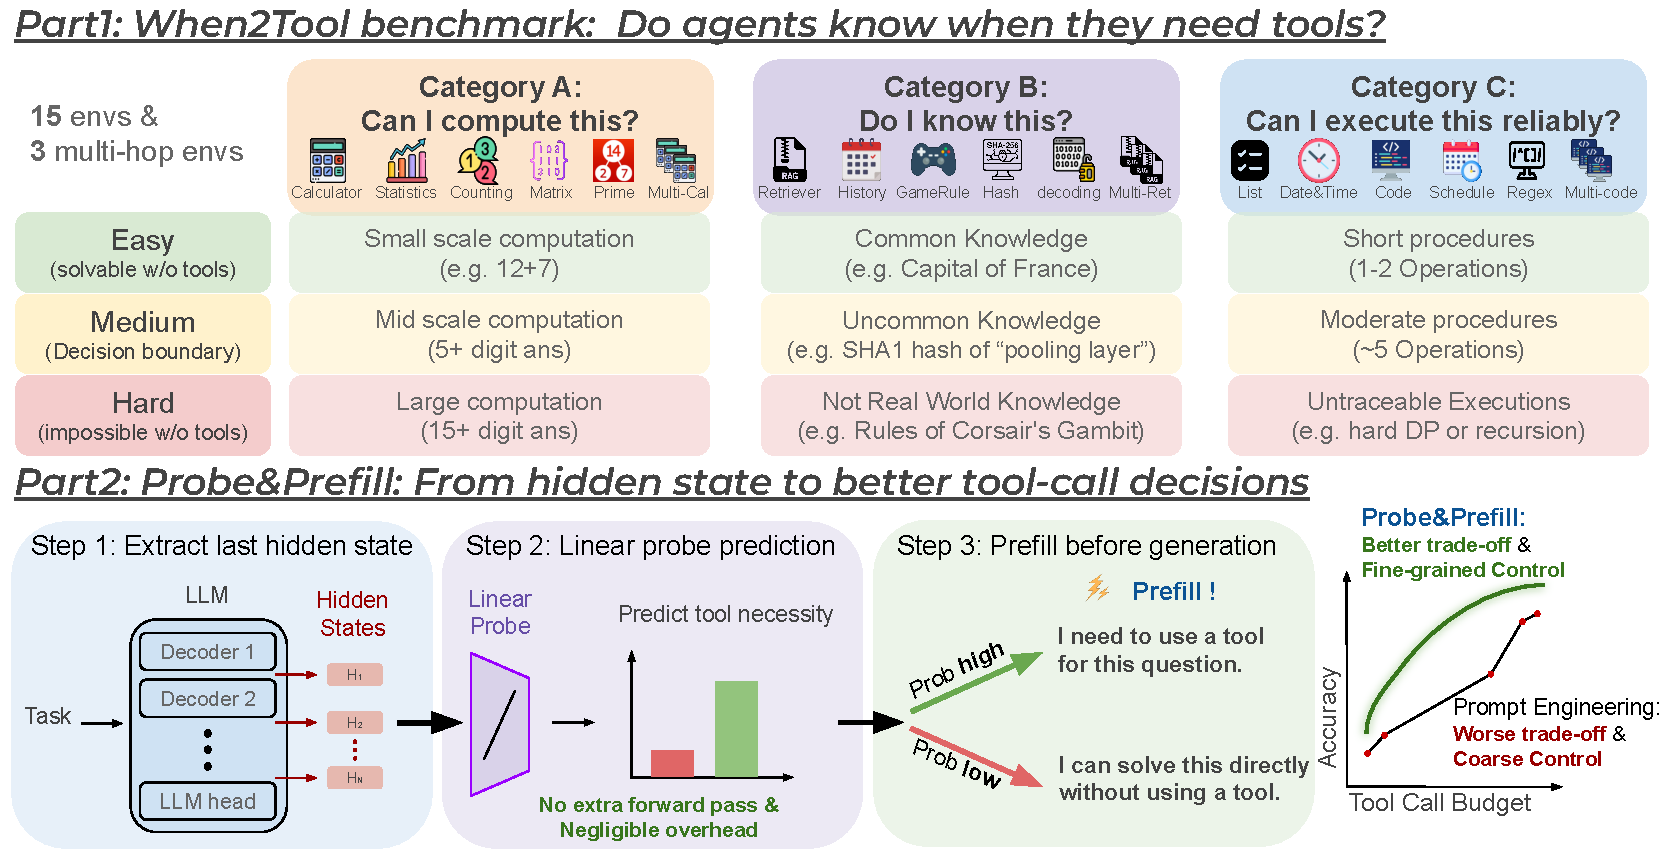
\includegraphics[width=\textwidth]{figures/overview.pdf}
\vspace{-15pt}
\caption{Overview. \textbf{Part 1}: We design \benchmark{} for studying whether LLM agents know when they need tools, spanning 15 single and 3 multi-hop environments across three categories, each with three difficulty levels. \textbf{Part 2}: \method{} reads the model's hidden state via a linear probe and prefills a steering sentence to guide the tool-call decision, achieving better tradeoffs.}
\vspace{-10pt}
\label{fig:overview}
\end{figure*}